\documentclass[11pt,aspectratio=1610,dvipsnames]{beamer}
\graphicspath{{figs/}}
\usetheme{default}
\usepackage{DasBeamerPaket}
\usepackage{animate}
\usepackage{lastpage}
\usepackage{tikz}
\setbeamercolor{section in toc}{fg=NavyBlue}
\setbeamercolor{frametitle}{fg=NavyBlue}
\captionsetup[figure]{labelfont=bf}
\captionsetup[table]{labelfont=bf}
\setbeamertemplate{caption}[numbered]
\newcommand{\btheta}{\boldsymbol{\theta}}
\begin{document}
\author{{\Large Dominic Schüchter}\\ \scriptsize \href{mail:dschuechter@uni-bonn.de}{\faEnvelope  \hspace*{0.1cm}dschuechter@uni-bonn.de} {\color{black}$|$} \href{https://github.com/dschuechter}{\faGithub  \hspace*{0.1cm}dschuechter}}
\title{Bayesian model selection}
\subtitle[Seminar physics760]{\textsc{Seminar physics760-Computational Physics}}
\logo{
\includegraphics[width=1cm]{UniBonnLogo}\vspace{235pt}\hspace{8pt}}

\date{\includegraphics[width=1.3cm]{institutelogo}\hspace{10px}
\includegraphics[width=1.3cm]{UniBonnLogo}}
\date{\includegraphics[width=8cm]{Titelbild.png}}
\definecolor{myWhite}{rgb}{1,1,1}

\setbeamertemplate{footline}[text line]{\parbox{0.3\linewidth}{\vspace*{-9pt}\textcolor{white} \insertsection  \hfill} \parbox{0.7\linewidth}{\vspace*{-8pt} \textcolor{white}{\hfill\hspace{-3cm}\insertshorttitle \phantom{ }-- \insertshortsubtitle}  \hfill \textcolor{myWhite}{\insertpagenumber/\pageref{LastPage}}}}

\addtobeamertemplate{footline}{ \makebox[0pt][l]{\hspace{-1cm}
		\raisebox{0cm}[0pt][0pt]{\colorbox{gray!15!black}{\phantom{{\large TEXTTEXTTEXTTEXTTEXTTEXTTEXTTEXTTEXTTEXTTEXTTEXTTEXTTEXTTEXTTEXTTEXTTEXTTEXTTEXTTEXTTEXTTEXTTEXTTEXTTEXTTEXTTEXTTEXTTEXTTEXTTEXTTEXTTEXTTEXTTEXTTEXTTEXTTEXTTEXT}}}}}}

\setbeamercovered{transparent}
\setbeamertemplate{navigation symbols}{}
\setbeamertemplate{frametitle}[default][left,leftskip=0.5cm]
%
\setbeamertemplate{itemize item}{\color{black}$\blacktriangleright$}
\setbeamertemplate{section in toc}[sections numbered]
\captionsetup{font=scriptsize,labelfont=scriptsize}

\AtBeginSection[]
{	
	\definecolor{myWhite}{rgb}{0,0,0}
	\begin{frame}[noframenumbering]
		\frametitle{}
		\addtocounter{page}{-1}
		\tableofcontents[currentsection]
		
	\end{frame}
\definecolor{myWhite}{rgb}{1,1,1}
}


\begin{frame}[plain]
	\setcounter{page}{0}
	\centering
	{\Large \color{MidnightBlue}{\textsc{Bayesian} model selection}}\\
	{\href{https://www.youtube.com/watch?v=oHg5SJYRHA0}{Seminar physics760 -- Computational Physics}}
	\vfill
	
	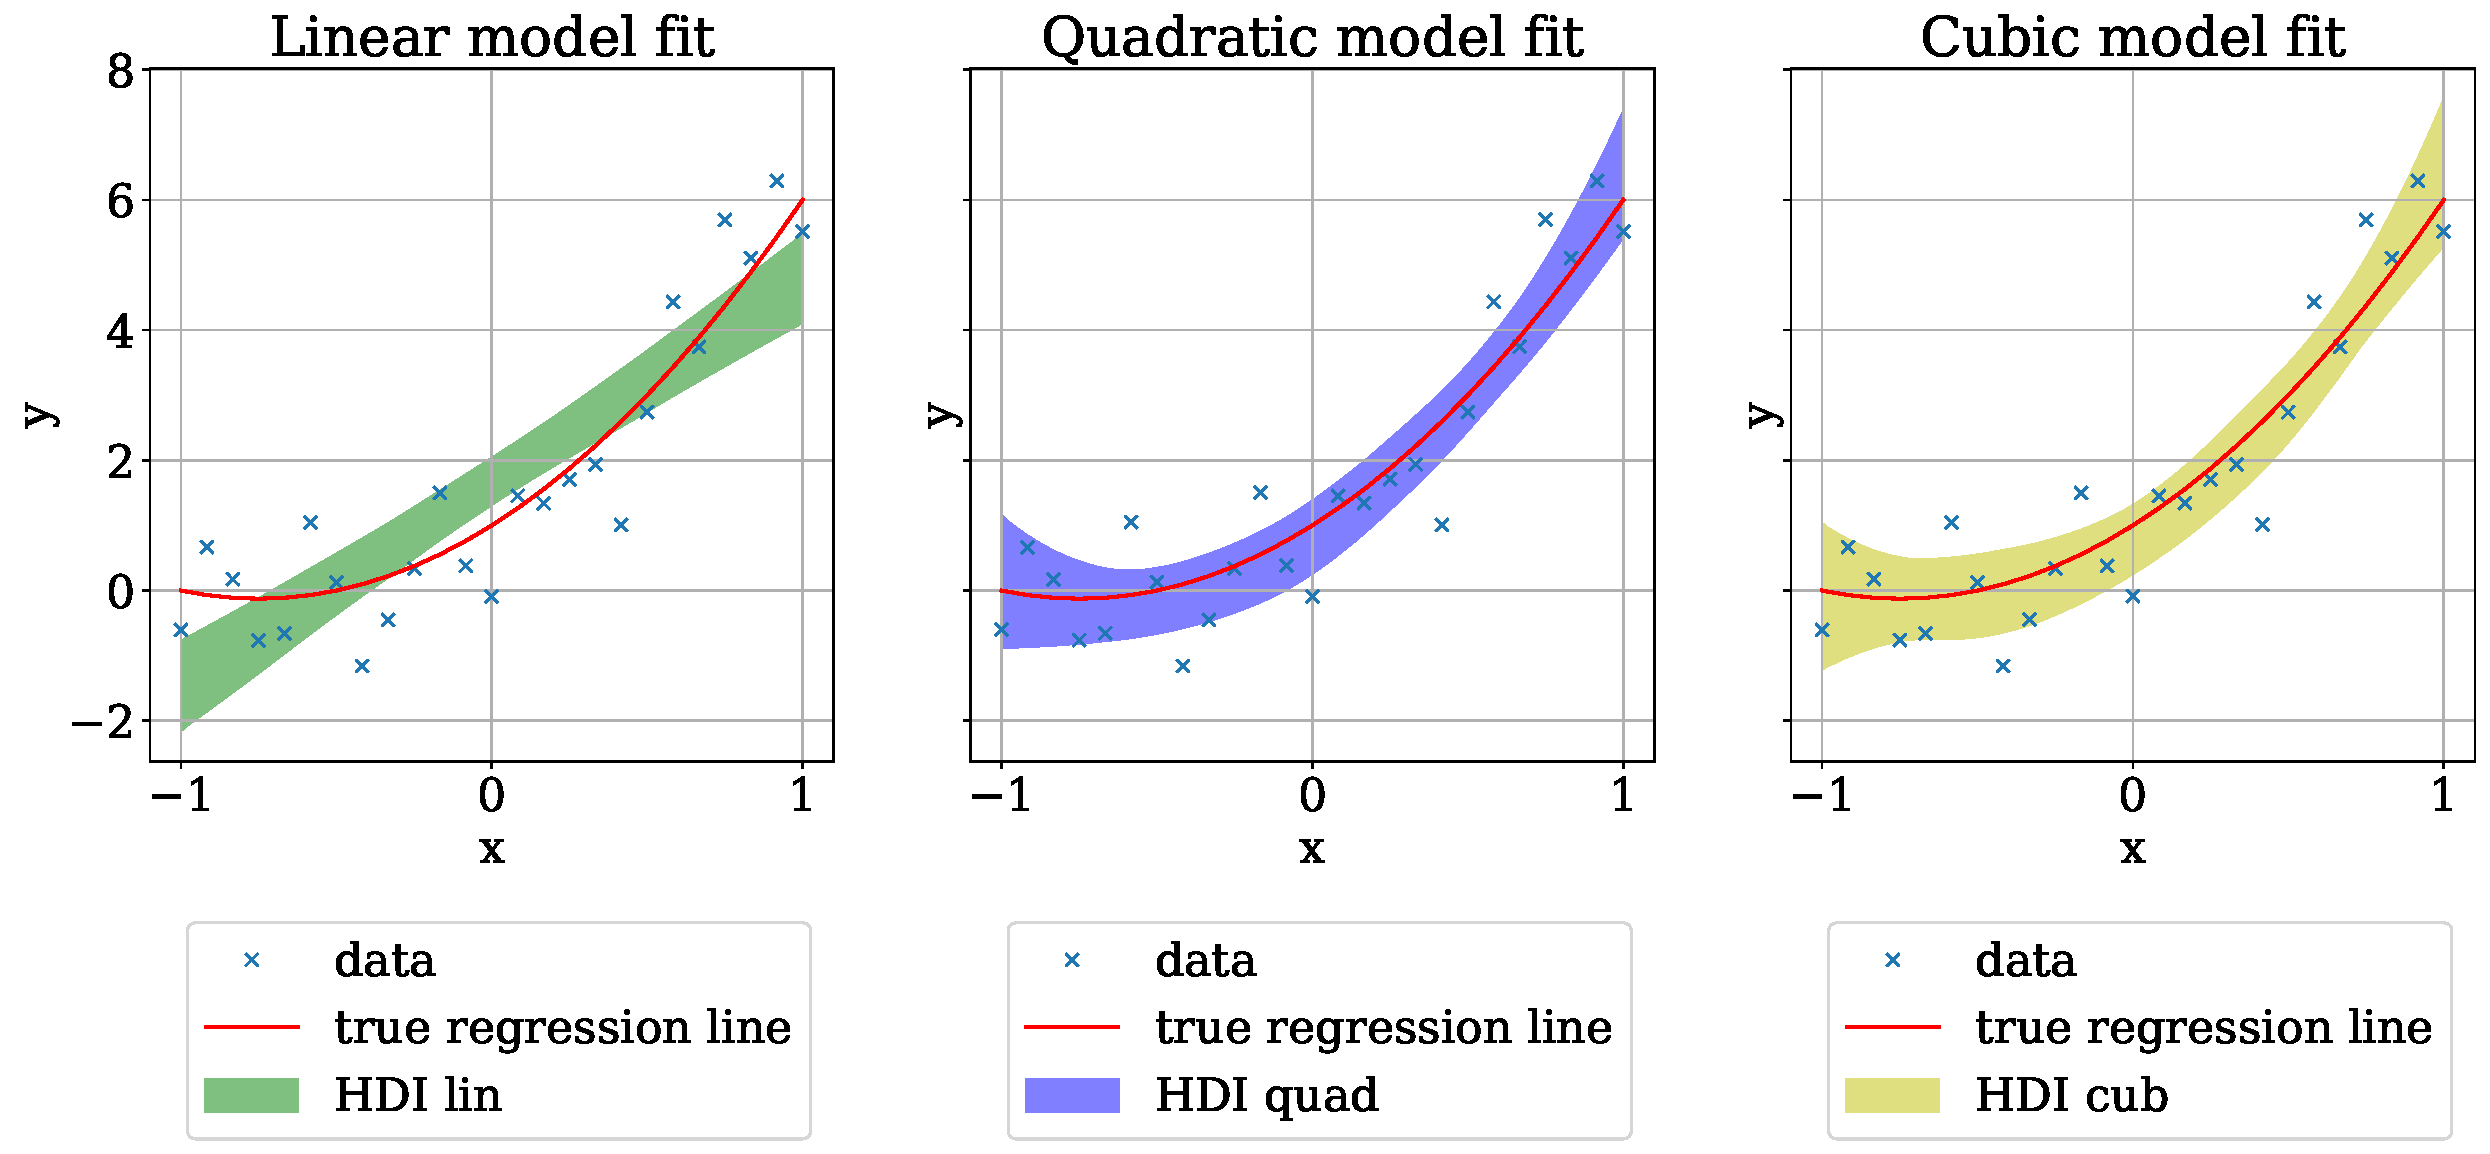
\includegraphics[width=0.8\linewidth]{figs/HDI_sigma_07a.pdf}
	\vfill
	\begin{minipage}{\linewidth}
		\centering
		\begin{minipage}{0.45\linewidth}
			\centering
			\textsc{Dominic Schüchter}\\
			\scriptsize \href{mailto:dschuechter@uni-bonn.de}{\faEnvelope  \hspace*{0.1cm}dschuechter@uni-bonn.de} {\color{black}$|$} \href{https://github.com/dschuechter}{\faGithub  \hspace*{0.1cm}dschuechter}\\
		\end{minipage}
%		$|$
		\begin{minipage}{0.45\linewidth}
			\centering
			\textsc{Jakob Krause}\\
			\scriptsize \href{mailto:krause@hiskp.uni-bonn.de}{\faEnvelope  \hspace*{0.1cm}krause@hiskp.uni-bonn.de} {\color{black}$|$} \href{https://github.com/krausejm}{\faGithub  \hspace*{0.1cm}krausejm}\\
		\end{minipage}
	\vspace{.5cm}
	
	Tutor: \textsc{Andreas Wirzba}\\
	\scriptsize \href{mailto:a.wirzba@fz-juelich.de}{\faEnvelope  \hspace*{0.1cm}a.wirzba@fz-juelich.de}
	\end{minipage}
	\vspace{0.2cm}
	
	19.03.2021
	 
	
%	  \makebox[0pt][l]{\hspace{-7cm}
%	 	\raisebox{0.2cm}[0pt][0pt]{%
%	 		
\includegraphics[width=2.5cm]{pics/UniBonnLogoWithTextMod.png} }}
 		
\end{frame}

%\begin{frame}[plain]
%	\maketitle
%	\setcounter{page}{0}
%\end{frame}

\section*{Introduction}
\begin{frame}{Introduction}
	\begin{tcolorbox}[colback=black!5,colframe=gray!15!black,title=\textsc{Bayes'} Theorem] 
		$$\text{prob}(\btheta|y)=p(\btheta|y)= \frac{p(y|\boldsymbol{\theta})\cdot p(\boldsymbol{\theta})}{p(y)}$$
		with
		\begin{itemize}
			\item \emph{posterior} $p(\btheta|y)$\\
			\item \emph{likelihood} $p(y|\boldsymbol{\theta})$\\
			\item \emph{prior} $p(\boldsymbol{\theta})$\\
			\item \emph{marginal likelihood} $p(y)=\int_{-\infty}^{+\infty}\text{d}\boldsymbol{\theta} p(y|\boldsymbol{\theta})p(\boldsymbol{\theta})$\\
		\end{itemize}
	\begin{center}
		\textbf{This can be used for \emph{model selection} (?)}
	\end{center}
\end{tcolorbox}
\end{frame}


\section*{Table of Contents}

\begin{frame}{Table of Contents}
	\tableofcontents
\end{frame}

\section{Theory}
\subsection{Parameter estimation}
\begin{frame}{Parameter estimation}
	\textsc{Jan} and \textsc{Marius} already talked about this, so here we only sketch the basics again
	\begin{equation}
		\label{eq:marp}
		p(\theta_i|y,M)=\int p(\boldsymbol{\theta}|y,M)\prod_{j\neq i}\text{d}{\theta_j}
	\end{equation}

\begin{align}
	\begin{split}
		p(\theta|y,M)=\max \Leftrightarrow \theta=\hat{\theta}\\
		\langle\theta\rangle=\int_{-\infty}^{\infty}\text{d}\theta  p(\theta|y,M)\cdot\theta
	\end{split}
\end{align}
\end{frame}

\subsection{Model comparison}
\begin{frame}{Model comparison}
	How do we turn \textsc{Bayes'} theorem into a tool for model comparison?
	\begin{tcolorbox}[colback=black!5,colframe=gray!15!black,title=\textsc{Bayes} factor] 
		\begin{equation}
			p(M_i|y)=\frac{p(M_i)\cdot p(y|M_i)}{p(y)}.
		\end{equation}
		\begin{equation}\label{eq:bf}
			O_{ij}:=\underbrace{\frac{p(M_i|y)}{p(M_j|y)}}_{\text{posterior odds}}=\underbrace{\frac{p(y|M_i)}{p(y|M_j)}}_{\text{\textsc{Bayes} Factor}}\cdot\underbrace{\frac{p(M_i)}{p(M_j)}}_{\text{prior odds}}=B_{ij}\cdot\frac{p(M_i)}{p(M_j)}.
		\end{equation}
	\end{tcolorbox}
\end{frame}
\begin{frame}{Model comparison}

	\begin{tcolorbox}[colback=black!5,colframe=gray!15!black,title=\textsc{Bayesian} complexity] 
		\begin{equation}\label{eq:Bayes_Complexity}
			\mathcal{C}_b=-2\int \text{d}\boldsymbol{\theta} p(\boldsymbol{\theta}|y,M)\log(\mathcal{L}(\boldsymbol{\theta}))+2\log(\mathcal{L}(\boldsymbol{\tilde{\theta}})),
		\end{equation}
	
		\begin{equation}\label{eq:Bayes_Complexity_alt}
		\mathcal{C}_b=\overline{\chi^2(\boldsymbol{\theta})}-\chi^2(\boldsymbol{\tilde{\theta}}),
	\end{equation}
	\end{tcolorbox}
\end{frame}
\section{Methods}

\subsection{Monte-Carlo-Sampling}
\begin{frame}{Monte-Carlo-Sampling}
	\begin{minipage}{\linewidth}
		\begin{minipage}{0.6\linewidth}
			\begin{tcolorbox}[colback=black!5,colframe=gray!15!black,title={Benefits of Monte-Carlo-Sampling}] 
				 \begin{equation}
					\langle \boldsymbol{\theta}\rangle\approx \int p(\boldsymbol{\theta} | y)\boldsymbol{\theta}d\boldsymbol{\theta}=\frac{1}{N}\sum_{t=0}^{N-1}\boldsymbol{\theta}^{(t)},
				\end{equation}
				 \begin{equation}
					\langle f(\boldsymbol{\theta})\rangle\approx\frac{1}{N}\sum_{t=0}^{N-1}f(\boldsymbol{\theta}^{(t)}).
				\end{equation}
			\end{tcolorbox}
		\end{minipage}
		\hfill
		\begin{minipage}{0.3\linewidth}
			\begin{figure}
				
\includegraphics[width=\linewidth]{arviz_logo}
				\vspace{0.1cm}
				
				
\includegraphics[width=\linewidth]{PyMC3_banner}
				\caption{\texttt{ArviZ} \cite{ArviZ} and \texttt{PyMC3} \cite{PyMC3}}
			\end{figure}
			
		\end{minipage}
	\end{minipage}
	
	
\end{frame}

\subsection{\textsc{Savage-Dickey}-Density-Ratio (SDDR)}
\begin{frame}{\textsc{Savage-Dickey}-Density-Ratio (SDDR)}
\end{frame}
\subsection{Error analysis and diagnostics}
\begin{frame}{Error analysis and diagnostics}
	Inhalt...
\end{frame}

\section{Examples}

\subsection{Coin-Flip}
\begin{frame}{Choosing priors and likelihoods}
	
\end{frame}

\begin{frame}{Computing \textsc{Bayes}-factor}
	
\end{frame}
\subsection{Fitting a polynomial of unknown degree}

\section{Summary}
\begin{frame}{Summary}
	\begin{tcolorbox}[colback=black!5,colframe=gray!15!black,title=, width=\linewidth]
		\begin{itemize}
			\item 
		\end{itemize}
	\end{tcolorbox}
\end{frame}

\section*{References}
\begin{frame}[allowframebreaks]{References}
	\setbeamertemplate{bibliography item}[text]

	\printbibliography
\end{frame}

\end{document}